\clearpage
\section{\textsc{Theoretische Grundlagen}}
\subsection{Radioaktive Zerfälle}
Instabile Kerne können unter Aussendung charakteristischer radioaktiver Strahlung zerfallen. Dieser Zerfall kann auf unterschiedlichen Wegen geschehen und dabei können unterschiedliche Arten von Strahlung frei gesetzt werden. Radioaktiver Zerfall ist ein statistischer Prozess, dabei ist die Änderung einer radioaktiven Probe $dN$ nach einer Zeit $t$ proportional zur gesamten Menge der Probe N:
\begin{center}
\[\frac{dN}{dt}=-\lambda N \]
\end{center}
Eine Lösung zu dieser Differentialgleichung erhält man durch separieren der Variablen und erhält durch integrieren:
\begin{center}
\[\ln N(t)-\ln N(0)= \int\limits_{N(t)}^{N(0)}\frac{dN'}{N'}=- \int\limits_{t}^{0}\lambda dt'= -\lambda t \]
\[ \Leftrightarrow \ln{\frac{N(t)}{N(0)}} = -\lambda t\]\\
\[ \Leftrightarrow N(t)= N(0) \exp(-\lambda t)\]
\end{center}
Aus dieser Formel lässt sich nun auch die Halbwertszeit $T_{\frac{1}{2}}$ berechnen:
\begin{center}
\[ \frac{1}{2}N_0 = N(T_{\frac{1}{2}}) = N_0 \exp(-\lambda T_{\frac{1}{2}})\]\\
\[ \Leftrightarrow T_{\frac{1}{2}} = \frac{\ln 2}{\lambda}\]
\end{center}
Und für die Lebensdauer gilt
\begin{center}
\[ \tau = \frac{1}{\lambda}= \frac{T_{\frac{1}{2}}}{\ln 2}~~. \]
\end{center}
\subsubsection{$\alpha$-Zerfall}
Bei schweren Kernen kann man das Phänomen des  $\alpha$-Zerfalls. Beim $\alpha$-Zerfall zerfällt der Mutterkern in den Tochterkern unter Aussendung eines Helium-4-Atomkerns:
\begin{center}
$_Z^AX \rightarrow _{Z-2}^{A-4}X+_2^4He$.
\end{center}
\subsubsection{$\beta$-Zerfall}
Es gibt drei verschiedene Arten von $\beta$-Zerfall: $\beta^+$- und $\beta^-$-Zerfall und den Elektroneneinfang (EC, Electron Capture).\\
~\\
\textbf{$\beta^+$-Zerfall:} Bei Kernen mit relativem Überschuss an Protonen kann $\beta^+$-Zerfall auftreten. Dabei wird ein Proton unter Aussendung eines Positrons und eines Neutrinos in ein Neutron umwandelt:
\begin{center}
$\mathit{_1^1p \rightarrow _0^1n + e^+ + \nu}$
\end{center}
Die Kernladung veringert sich um eins. Das Positron wird sich nach seiner Abbremsung durch Materie bald mit einem Elektron zu einem Positronium-Atom vereinigen, welches nach einer mittleren Lebensdauer von $10^{-7}$s bis $10^{-9}$s in zwei $\gamma$-Quanten zu je 511keV zerfällt.\\
~\\
\textbf{$\beta^-$-Zerfall}: Bei Kernen mit relativem Überschuss an Neutronen kann $\beta^-$-Zerfall auftreten. Hierbei wandelt sich ein Neutron in ein Proton um, unter Aussendung eines Elektrons und eines Antineutrinos, welches ein Teil der Zerfallsenergie weg trägt:
\begin{center}
$\mathit{_0^1n \rightarrow _1^1p+e^- + \overline{\nu}}$
\end{center}
Die Kernladung verringert sich um eins. Die Energie der ausgesendeten Elektronen ist kontinuierlich verteilt.\\
~\\
\textbf{Elektroneneinfang (EC, Electron Capture)}: Vor allem bei schweren Kernen mit Protonenüberschuss tritt EC auf. bei diesem Effekt wird ein Elektron aus der K-Schale vom Kern eingefangen unter Aussendung eines Neutrinos, wodurch sich die Kernladungszahl um eins verringert. Der dadurch entstandene freie Platz in der K-Schale wird durch ein Elektron aus der, meistens nächst höheren L-Schale wieder aufgefüllt. Die durch den Übergang des Elektrons in die niedrigere Schale frei werdende Energiedifferenz wird als Röntgen- oder Augerstrahlung abgestrahlt. Der freie Platz in der L-Schale wird wiederum durch ein Elektron aus einer höheren Schale besetzt. Dieser Prozess setzt sich in Richtung äußerer Schalen fort bis eine stabile Elektronenkonfiguration wieder erreicht ist. Bei diesem Vorgang wird bei jedem Elektronenübergang eine für die entsprechende Energiedifferenz charakteristische Röntgenstrahlung frei gesetzt.
\subsubsection{$\gamma$-Strahlung}
Bei der $\gamma$-Strahlung haben wir keine Veränderung bei der Nukleonenzahl oder der Kernladungszahl. Sie ist eine Begleiterscheinung der oben genannten Zerfälle. Nach einem Zerfall ist der Tochterkern meist in einem angeregten Zustand, welcher unter aussenden von $\gamma$-Quanten, mit der entsprechenden Energie, in einen tieferen Zustand zurück fällt bis er beim Grundzustand angekommen ist.
\subsubsection{Innere Konversion (IC, Internal Conversion)}
Ein zur $\gamma$-Strahlung konkurrierender Prozess ist die innere Konversion. Sie tritt vor allem bei schweren Kernen und geringer Zerfallsenergie auf. Die innere Konversion ist ein strahlungsloser Übergang eines angeregten Kernzustands in einen tieferen, hier wird die freiwerdende Energie an eines der Hüllenelektronen übertragen und dieses bei diesem Vorgang ausgesendet wird. Die Energieübertragung findet hierbei direkt statt ohne dass ein reelles $\gamma$-Quant erzeugt wird welches das Elektron später absorbiert. Diese Elektronen zeigen, im Gegensatz zum $\beta$-Zerfall, ein kontinuierliches Spektrum. Man erhält ein monoenergetisches Spektrum welches von der Schale des emittierten Elektrons abhängt. Die frei werdende Energie bei auffüllen der Lücke, durch herabfallende Elektronen in Hüllen niedrigerer Energien, wird als charakteristische Röntgenstrahlung oder durch Auger-Elektronen aufgefüllt.
\subsection{Prozesse in der Atomhülle}
Wie bereits besprochen ist die Folge eines Elektroneneinfangs oder einer inneren Konversion, ein unbesetzter Elektronen-Zustand. Dieser Zustand wird durch ein Elektron aus einer höheren Schale aufgefüllt. Durch den Übergang wird die frei werdende Energiedifferenz entweder durch Emission von charakteristischer Röntgenstrahlung oder durch ein Auger-Elektron abgeführt. Beim Effekt des Auger-Elektrons wird die Energie wie bei der inneren Konversion direkt an das Elektron einer anderen Schale übertragen, welches dann druch aus der Atomhülle geschlagen wird. Dieses Elektron nennt man Auger-Elektron. Die nun frei gewordene Lücke wird nun wieder durch ein Elektron besetzt unter Aussendung von Röntgenstrahlung oder eines Auger-Elektrons.
\subsection{Wechselwirkung von Photonen mit Materie}
Man nutzt die Wechselwirkung von $\gamma$-Quanten mit Materie um diese Nachzuweisen. $\gamma$-Strahlen befolgen bei der Absorption folgendes Exponentialgesetz:
\begin{center}
$I_d=I_0e^{\mu d}$
\end{center}
Wobei $I_0$ der Intensität vor dem absorbierenden Material entspricht, $I_d$ der Intensität bei einer Eindringtiefe $d$ und $\mu$ ist der Absorptionskoeffizient der absorbierenden Materie. Dieser Koeffizient hängt sowohl von $E_{\mu}$ als auch vom Absorber-Material ab.
Es gibt im Wesentlichen drei Wechselwirkungs-Mechanismen von $\gamma$-Quanten mit Materie deren Wirkungsquerschnitt mit der $\gamma$-Energie $E_{\gamma}$ und der Kernladungszahl $Z$ des Materials abhängt:
\subsubsection{Photoeffekt}
Der Photoeffekt tritt vor allem bei einer Energie $E_{\mu}$ < 200 keV (bei $Z \approx 50$) auf. Beim Photoeffekt überträgt ein $\gamma$-Quant seine Energie vollständig an ein Elektron, worauf dieses aus der Atomhülle geschlagen wird und erhält kinetische Energie. Die frei Stelle in der Atomhülle wird durch ein Elektron aus einer höheren Schale besetzt was zu den oben genannten Effekten führt.
\subsubsection{Comptoneffekt}
Der Comptoneffekt tritt überwiegend bei einer Energie von 200 keV < $E_{\gamma}$ < 5 MeV auf. Beim Comptoneffekt gibt ein $\gamma$-Quant beim Zusammenstoß mit einem Elektron nur ein Teil seiner Energie an das Elektron ab. Es wird an dem Elektron gestreut.

\begin{figure}[h]
\begin{center}
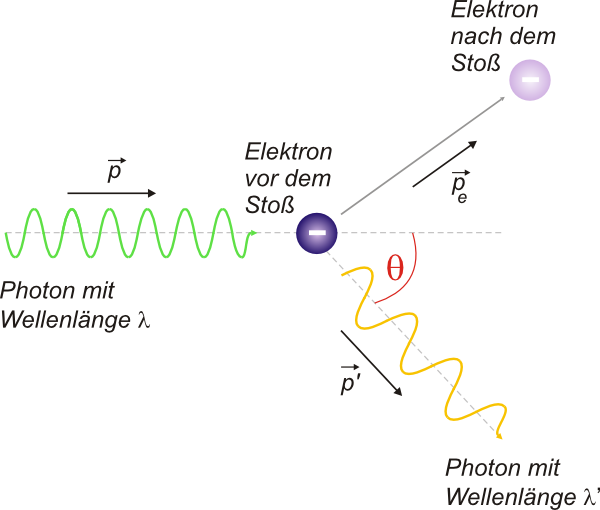
\includegraphics[scale=0.25]{compton}
\caption{Schema zum Comptoneffekt. Quelle: [ung]}
\label{fig:graph1}
\end{center}
\end{figure}

\subsubsection{Paarbildung}
Paarbildung beobachtet man ab einer Energie $E_{\gamma} \ge$ 1,022 MeV. Paarbildung erhält man, wenn ein $\gamma$-Quant mit einem elektromagnetischen Feld eines Atomkerns oder eines Elektrons in Wechselwirkung tritt. Dabei wird das $\gamma$-Quant vollständig absorbiert und ein Positron-Elektron-Paar entsteht. Die Energie des $\gamma$-Quants wird auf die beiden Teilchen verteilt und der überschüssige Impuls wird vom Kern aufgenommen. Das Positron zerfällt zu zwei $\gamma$-Quanten mit je 0,511 MeV, da es nicht lange existieren kann und sich mit einem Elektron vereint.
\subsection{Elektronik zum Nachweis vom $\gamma$-Quanten}
\subsubsection{Szintillator}
Um $\gamma$-Quanten zu detektieren benutzen wir einen Szintillator. Generell unterscheidet man hier zwischen zwei Arten von Szintillatoren, den anorganischen und den organischen. In unserem Aufbau wird ein anorganischer Szintillator benutzt.\\
Im Gegensatz zu den organischen, bei denen die einzelnen Moleküle eine Rolle spielen, spielt bei den anorganischen das Gitter des Ionenkristalls eine Rolle. Bei beiden Arten erhält man jedoch durch die Interaktion von einem $\gamma$-Quant mit dem Detektormaterial eine Lichtemission. Dabei wird ein $\gamma$-Quant mit hoher Energie umgewandelt zu einem oder mehreren mit geringerer Energie, durch den Photo- oder Comptoneffekt. Unsere Szintillator enthält einen NaI(Ti)-Kristall, die Dotierung mit Titan sorgt für weitere Energieniveaus in der Bandlücke des reinen NaI-Kristalls und somit, dass die Quanten mit bereits kleinerer Energie nicht wiederholt vom Kristall absorbiert werden.
\subsubsection{Photomultiplier}
Der Photomultiplier wandelt Lichtimpulse, in unserem Fall die vom Szintillator zugeleiteten, umzuwandeln in zur Lichtintensität proportionale elektrische Impulse umzuwandeln und diese durch Elektronenvervielfachung zu verstärken. Zum Umwandeln des der Lichtimpulse wird eine Photokathode benutzt. An ihr schlagen die ankommenden $\gamma$-Quanten, durch den Photoeffekt, Elektronen heraus. Ein $\gamma$-Quant kann mehrere Elektronen aus der Photokathode heraus schlagen welche durch eine anliegende Spannung zu ersten Dynode beschleunigt und befreien dort beim aufschlagen mehrere Sekundärelektronen, welche zur zweiten Dynode beschleunigt werden. Dies wiederholt sich bei allen weiteren Dynoden, da bei diesen sich jeweils die Spannung erhöht.

\begin{figure}[h]
\begin{center}
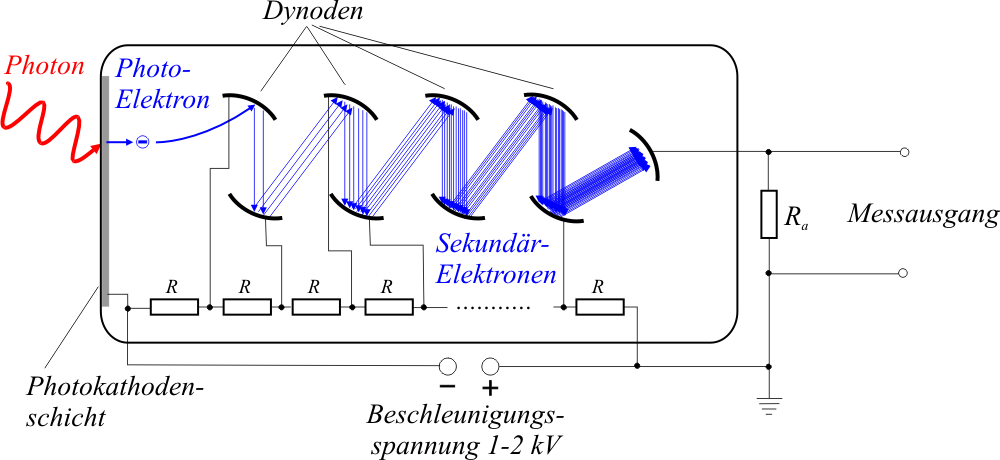
\includegraphics[scale=1.0]{PM}
\caption{Prinzipielle Funktionsweise eines Photomultipliers. Quelle: [hep].}
\label{fig:PM}
\end{center}
\end{figure}


